\section{Durchführung}
\label{sec:Durchführung}

Der Versuchsaufbau ist in Abbildung (2) zu sehen.
\begin{figure}[H]
  \centering
  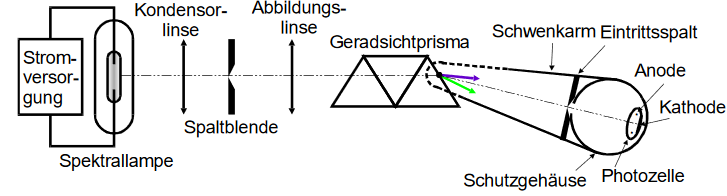
\includegraphics[height=4cm]{aufbau.PNG}
  \caption{Versuchsaufbau zur Analyse des Photoeffekts. \cite{kent}}
\end{figure}
Das Licht einer Spektrallampe wird durch eine Kondensatorlinse gebündelt, durch eine Spaltblende und eine Linse geschickt, und fällt in ein Prisma, um die Spektrallinien des Lichts zu trennen.
Die Photozelle(s. Abbildung (3)), aus der die Elektronen emittiert werden, besteht aus einem Glaskolben mit einer Photokathode und einem Anodendraht. 
\begin{figure}[H]
  \centering
  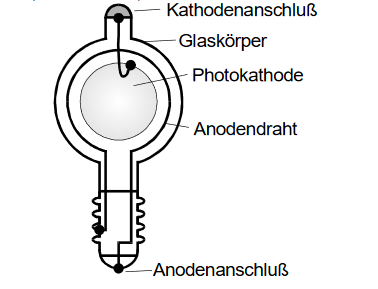
\includegraphics[height=6cm]{photo.PNG}
  \caption{Darstellung einer Photozelle. \cite{kent}}
\end{figure}
An die Photozelle wird eine Spannung angelegt, durch die die Elektronen abgebremst werden, und welche mit einem Digitalvoltmeter eingestellt werden kann. Um den Strom zwischen Kathode und Anode zu messen wird ein Picoamperemeer angeschlossen(s. Abbildung (4)). 
\begin{figure}[H]
  \centering
  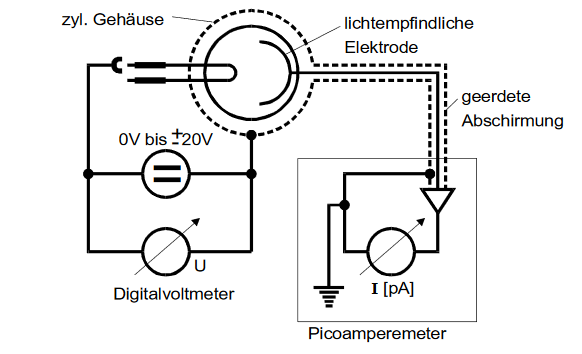
\includegraphics[height=6cm]{schaltung.PNG}
  \caption{Schaltung zur Gegenfeldmethode. \cite{kent}}
\end{figure}
Die Elemente der Apparatur müssen richig einjustiert werden, sodass die Linien der Farben deutlich erkennbar sind. Dann wird die Apparatur so ausgerichtet, dass erst gelbes, dann grünes, blaugrünes, und ein starkes und ein schwaches violett auf die Photozelle fallen.
Dann wird die Spannung bis hin zum Wert, bei dem die Strömstärke Null ist, in sinnvollen Schritten eingeregelt und die zugehörige Stromstärke gemessen.
Dies wird für alle aufgelisteten Farben wiederholt.
Zuletzt wird der Photostrom erneut für gelbes Licht gemessen; diesmal im Bereich von -20V - 20V. Somit muss das Voltmeter einmal umgepolt werden, damit nicht nur eine Gegenspannung, sondern auch eine Beschleunigungsspannung eingestellt werden kann.